\section{BioMérieux Biopedia}
\label{biomerieuxBiopedia}

\begin{figure}[h]
    \centering
    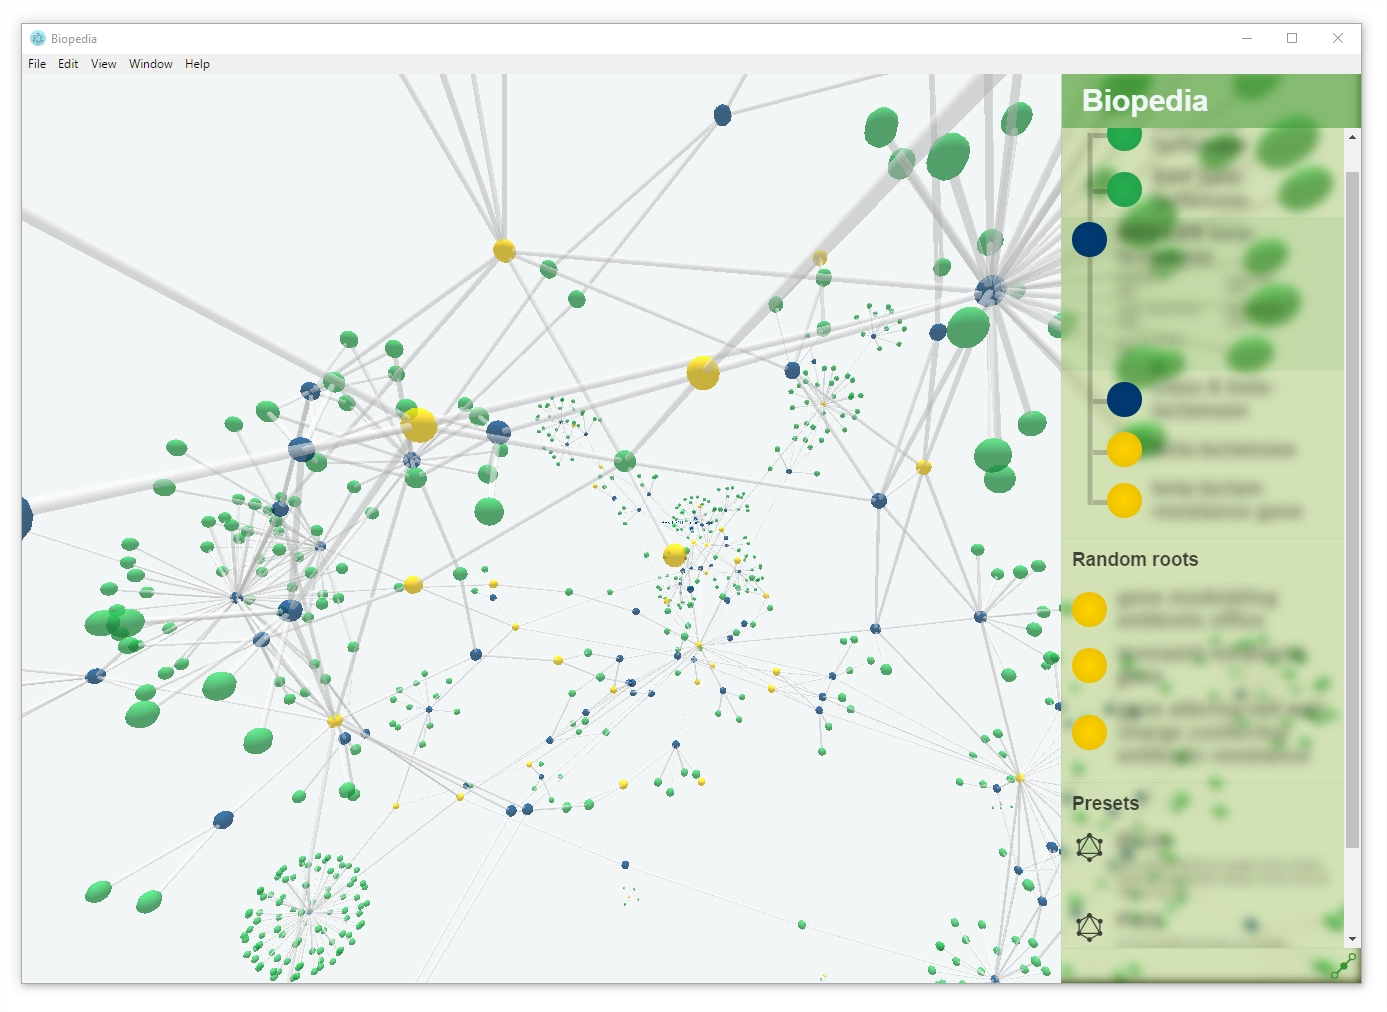
\includegraphics[scale=0.35]{img/Biopedia.jpg}
    \caption{Capture d'écran de la version actuelle de Biopedia}
\end{figure}

Biopedia est un projet de longue date pour LTBL .
L'objectif de cette application est de présenter les données d'une base de données de BioMérieux sous forme de graph pour la présentation aux clients interessés.

Au momment où j'ecrit ces lignes, je sous toujours en train de développer activement cette application pour la présenter au client final le 20 Avril;
Certaines informations pourront alors changer à l'avenir.

\subsection{Application précédente}
\label{biomerieuxBiopediaApplicationPrécédente}

Cela longtemps que LTBL à ce projet de visualisation de graphs et une première version à déjà été présentée.
Mais cette application se basait sur une vielle librairie et de nouvelles fonctionnalités ont été demandées par le client.

Apres, uyne étude du code de cette application nous avons décidé de revoir complètement son code.
Je me suis donc lancé sur la creation d'une tout nouvelle application de visualisation.

Cette application devra disposer des fonctionnalités suivantes :

\begin{itemize}
    \item Afficher les données dans un graph en 3 dimentions
    \item Afficher les nom des doeuds du graph quand on clique dessus
    \item Afficher les parents et enfant de ce noeud lors de la selection
    \item Aisément naviguer dans les données
    \item Afficher une potion du graph uniquement dans le cadre d'une étude de cas
\end{itemize}

\subsection{Téchnologies}
\label{biomerieuxBiopediaTéchnologies}

Pour créer cette application, je me souis tout d'abord tourné vers Unity\footnote{Unity est un moteur de jeu permettant d'afficher dans une scene en 3D des structures associés à des materiaux.} pour la creation d'un environnement en 3 dimentions.
Unity permet d'avoir des environnnements 3D tres interactifs et facile à utiliser.
Mais j'ai aussi remarqué un manque évident de librairies permettant de créer des graphs comme dans l'ancienne version de biopedia.
De plus, je n'allait pas passer les 3 semaines dédiés à ce projet pour la recréation d'une graphique de ce type.

J'ai donc décider de retourner sur une solution Web avec Electron et ls Webcomponents.
Pour ce faire, j'ai utilisé la librairie \emph{3d-force-graph} se basant sur \emph{ThreeJS} pour l'affichage en 3D dans un canvas WebGL.

\emph{ThreeJs} est la principale librairie permettant de concevoir des scenes en 3D avec WebGL .
Elle permet de placer des primitives dans la scene 3D et de faire diverses actions comme des mouvements de camera, l'utilsiation de materianx et la creation d'animations.
Dans mon cas, je l'utilise pour représenter le graphique des données.

\subsection{Force-directed graph}
\label{biomerieuxBiopediaForceDirectedGraph}

Les données de BioMérieux sont des données réparties en Graph.
Cela signifie que ce sont des données représentés par un ensemple de \emph{Noeuds} reliés ensemble par des \emph{Relations}.
les relations de ce graph sont orientées, c'est a dire qu'elles disposent d'un noeud source et d'un noeud cible.
Ce type de graph peut être représenter de multiples manières mais la technique que j'ai utilisé ici est la technique du \emph{Force-directed Graph}.

Cette technique consiste à considèrer chaque noeud comme un objet physique dans l'espace (ou le plan suivant le nombre de dimentions) et chaque relation comme un ressort reliant les noeuds.
On applique alors des forces sur les noeuds et on applique les lois de la physique au fil du temps pour obtenir un rendu graphiquement plaisant.
Cela peut prendre un certain temps avant d'avoir un resultat satisefaisant car ce système est itératif.
Il nécéssite alors une évolution du graph jusqu'a atteindre un etat de stabilité.

Je me suis interessé à la simulation de ce genre de système pour l'implémenter dans Unity mais due a une deadline assez proche, j'ai été obligé de trouver une librairie proposant une simulation de la position des noeuds.

\subsubsection{Nomenclature}
\label{biomerieuxBiopediaNomenclature}

Le graph de biomérieux dispose d'une nomenclature spécifique permettant de repèrer les différents éléments.
Dans notre cas, les couleurs montrent la position des noeuds dans l'arboréscense et non un type particulier.

\begin{description}
    \item[Neud vert] Représente une feille du graph soit un noeud qui ne dispose que de relations dans sa direction et aucune raltion ne partant de ce noeud
    \item[Neud bleu] Représente un noeud intérmediere soit un oeud disposant de relations depuis et vers lui
    \item[Neud jaune] Représente un noeud racine soit un neud qui ne dispose d'aucune relation dans sa direction
\end{description}

Chaque noeud de biopedia dispose de métadonnés donnat plus d'informations sur le noeud actuellement séléctionné.

\subsection{Structure}
\label{biomerieuxBiopediaStructure}

\begin{figure}[h]
    \centering
    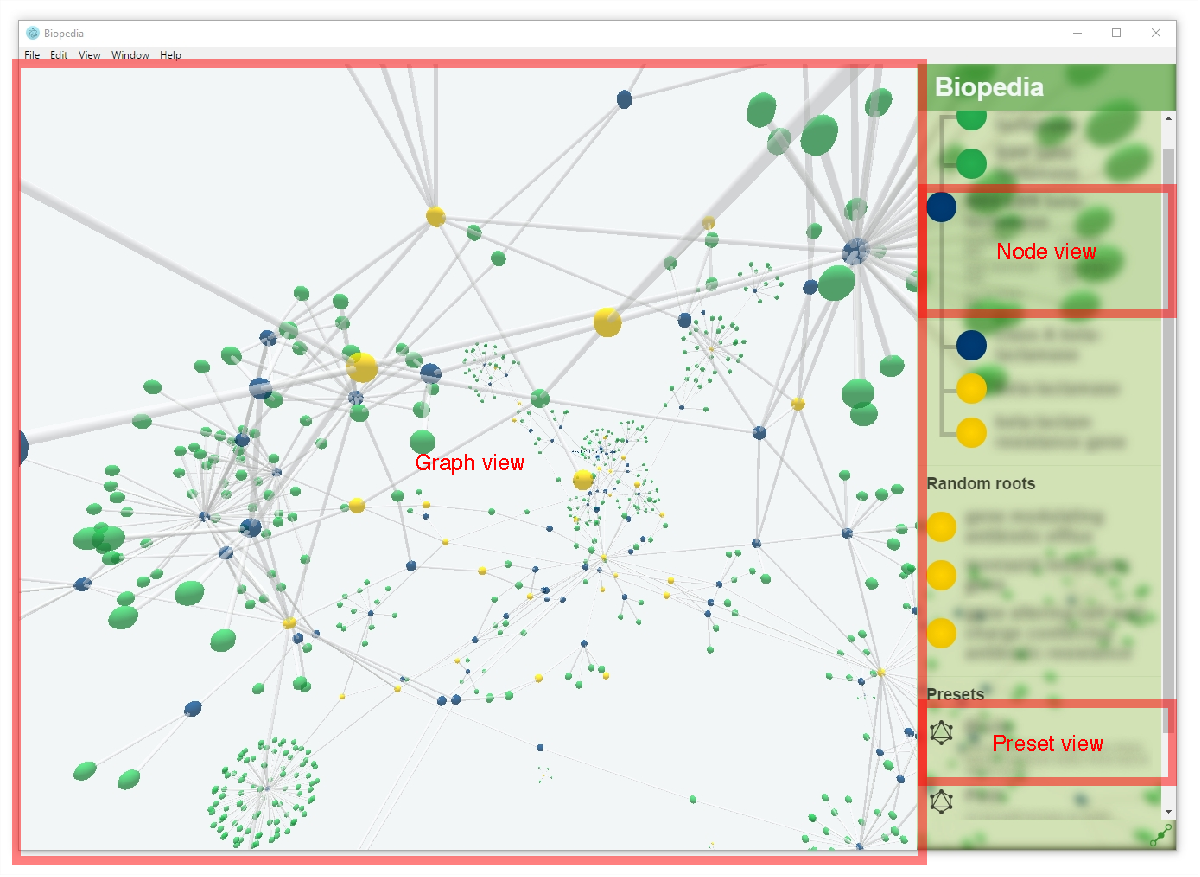
\includegraphics[scale=0.8]{img/biopedia-structure.pdf}
    \caption{Structure de l'application Biopedia}
\end{figure}

Dans cette application, j'utilise toutes les compétences acquises durant les projets précédents pour concevoir cette application de manière flexible pour qu'il soit aisé de comprendre mon code et d'ajouter des fonctionnalités à l'avenir.

\clearpage

Le différents components composant cetta pplication sont les suivants :

\paragraph{Graph view} Le lecteur de graphique permettant d'afficher un graphque des données en 3 dimentions a l'aide de \emph{ThreeJs}.
Il est possible de cliquer sur les noeuds du graphique pour le selectionner et afficher diverses informations dans la barre de contrôle présente sur la droite de l'interface.

\paragraph{Node view} En charge de formater l'affichage d'un noeud sur l'interface.
Ce component est totalement indépendant des autres et permet juste d'afficher un noeud avec un design constant.
Il est utilisé pour afficher le noeud séléctionné avec les diverses métadonnées qui lui sont associés dans la barre de contrôle.
Mais il est aussi utilisé dans la liste de noeuds aléatoire permettant de rapidement démarrer une navigation dans le graphique.

\paragraph{Prset view} Dans le même objectif d'unifier le design de l'affichage des différents preset, ce component sert à afficher un preset a l'utilisateur.
Il est utilisé dans la barre de contrôle et permet de séléctionner un preset pour filtrer l'affichage des données dans le graph.

\subsection{Conclusion}
\label{biomerieuxBiopediaConclusion}

Ce projet n'étant pas ecore fini, certaines informations et strucures peuvent changer.
Mais ce projet m'a permis de revoir mon évolution et les compétences acquises durant mon stage.
De plus j'ai eu l'occasion de découvrir la 3D dans le navigateur avec ThreeJs et les simulations de grahiques en 3 dimentions.
Ce projet fut très instructif et unique comme tout les projets chez LTBL.